\documentclass[12pt,a4paper]{report}

\usepackage[italian]{babel}
\usepackage{newlfont}
\usepackage{graphicx,  caption}
\usepackage{version}
\usepackage{chngcntr}
%\usepackage{float}
\usepackage{listings}

\usepackage{floatrow}
\usepackage{float}


\textwidth=450pt\oddsidemargin=0pt

\begin{document}

\begin{titlepage}
\begin{center}
{{\Large{\textsc{Alma Mater Studiorum $\cdot$ Universit\`a di
Bologna}}}} \rule[0.1cm]{15.8cm}{0.1mm}
\rule[0.5cm]{15.8cm}{0.6mm}
{\small{\bf DIPARTIMENTO DI INFORMATICA – SCIENZA E INGEGNERIA\\
Corso di Laurea in Ingegneria e Scienze Informatiche }}
\end{center}
\vspace{15mm}
\begin{center}
{\LARGE{\bf PARALLELIZZAZIONE SU GPU}}\\
\vspace{3mm}
{\LARGE{\bf ALGORITMO MARCHING SQUARES}}\\
\vspace{3mm}
{\LARGE{\bf PER APPLICAZIONE INDUSTRIALE}}\\
\vspace{25mm}

Elaborato in:\\
High Performance Computing\\
\end{center}
\vspace{25mm}
\par
\noindent
\begin{minipage}[t]{0.47\textwidth}
{\large{\bf Relatore:\\
Chiar.mo Prof.\\
Moreno Marzolla\\}}
{\large{\bf \\Correlatore:\\
Dott.\\
Matteo Roffilli}}
\end{minipage}
\hfill
\begin{minipage}[t]{0.47\textwidth}\raggedleft
{\large{\bf Presentata da:\\
Alessandro Sciarrillo}}
\end{minipage}
\vspace{30mm}
\begin{center}
{\large{\bf 
%Sessione\\%inserire il numero della sessione in cui ci si laurea
Anno Accademico 2022/2023}}%inserire l'anno accademico a cui si Ë iscritti
\end{center}
\end{titlepage}

\tableofcontents

\chapter{Abstract}
% una vista rapida della tesi 1/2 facciate, cosa si andrà a fare, quale è il problema, cosa si fa per risolverlo e quali risultati si otterranno. 
% keyword: cosa siANDRà a fare, OTTERREMO
Marching Squares(MS) é un algoritmo per la generazione di contorni in un campo scalare bidimensionale che viene ampiamente utilizzato nel Machine Vision in ambito industriale. Nella applicazione pratica in questione viene utilizzato su fotografie scattate da macchine per la selezione automatica della frutta per trovare i contorni di aree dell'immagine dove vengono riconosciuti dei difetti nel frutto. L'algoritmo viene applicato all'output di una CNN (Convolutional Neural Network) che é composto da una mappatura dei pixel dell'immagine in input nella rispettiva probabilità di appartenere ad una certa classe di difetto, vengono costruiti i contorni delle aree che hanno una probabilità maggiore di una certa soglia di contenere una certa classe. Le classi di difetto sono ad esempio: marcio, ruggine, danno da grandine fresca, danno da grandine cicatrizzato, danno da raccolta, danno da trasporto ecc.. \newline
Per ogni frutto che deve essere smistato correttamente dalle macchine in base alle sue condizioni vengono scattate più foto mentre viene trasportato su dei rulli che lo fanno roteare e permettono quindi alle fotocamere di raccogliere un insieme di scatti in cui il frutto é stato catturato in tutte le sue facce. Per ognuna delle foto scattate al frutto vengono generate delle matrici di probabilità per ogni classe di difetto, il risultato del processo di selezione é quindi l'insieme delle immagini dei vari lati di quel preciso frutto con i vari difetti racchiusi da un contorno che li identifica. \newline 
La costruzione di questo contorno viene attualmente effettuato da Python tramite il metodo \verb|findContours| della libreria skimage che utilizza un'implementazione seriale dell'algoritmo Marching Squares, lo scopo di questa ricerca é di implementare una versione parallela su GPU dell'algoritmo in modo da ridurre i tempi di esecuzione che risultano un fattore di importanza fondamentale.  Infatti ogni frazione di secondo risparmiata può essere utilizzata per aumentare il numero di frutti classificati in un'unità di tempo o per dedicare quel tempo ad altre elaborazioni utili a migliorare il risultato. 
Il metodo \verb|findContours| di skimage é scritto in Python ma la parte principale in cui utilizza MS é stata scritta in Cython (codice Python-like che viene compilato in codice C) per migliorare i tempi di esecuzione, può essere quindi considerata come una versione seriale già particolarmente ottimizzata. \newline L'obbiettivo è di parallelizzare proprio la stessa parte dell'algoritmo che skimage mantiene in Cython che è anche l'unica porzione di codice parallelizzabile dell'algoritmo MS. \newline
Le principali strategie che verranno esplorate sono:
\begin{itemize}
\item utilizzo dell'ultima versione di nvc++ per la parallelizzazione in fase di compilazione del codice Cython
% \item utilizzo delle direttive OpenMP per la parallelizzazione del codice C derivato dal codice Cython
\item utilizzo delle API Cuda-Python per il lancio di kernel Cuda (scritti manualmente) da Python 
\end{itemize}
Il metodo migliore che verrà poi utilizzato per la soluzione finale sarà quello che sfrutta le API Cuda-Python e i kernel Cuda scritti manualmente, riuscirà infatti ad ottenere uno Speedup di circa x5**[NOTA: sulla mia macchina,  attendo test su server azienda per aggiornare valore e inserire specifiche macchina] %TODO scrivere specifiche macchina
 rispetto al corrispondente codice seriale della libreria skimage. Verrà anche analizzato l'overhead nel lancio dei kernel Cuda introdotto da Python rispetto a una versione scritta in C. \newline
Nella soluzione finale viene inoltre implementata una elaborata versione parallela di exlusive scan composta da più kernel che risulta di particolare interesse nell'ambito dell'High Performance Computing.

\chapter{Introduzione alla programmazione Parallela}
% guardare altre tesi per vedere in che ordine metterlo
% valutare se tenerlo o meno

\chapter{Introduzione e Analisi del Problema}
\section{Introduzione}
% spiegare il problema e la sua utilità, obbiettivo
\subsection{Marching Squares (MS)} %valutare di farlo diventare capitolo
L'algoritmo Marching Squares genera contorni per un campo scalare a due dimensioni, data una matrice di valori e una soglia é in grado di trovare un insieme di segmenti che delimitano le aree della matrice in cui il valore contenuto dalle singole celle é maggiore della soglia data. \newline
Una delle elaborazioni più utilizzate viene effettuata considerando separatamente ogni gruppo di quattro elementi della matrice disposti a forma di quadrato, ognuno di questi quadrati può ricadere in uno di sedici diversi casi possibili ben definiti. Per definire a quale tipo appartiene un certo quadrato bisogna prima binarizzare i valori dei quattro spigoli in base alla soglia data, la posizione dei valori negli spigoli é importante poiché i sedici casi sono definiti con un'orientazione ben precisa. Nella figura 3.1 é possibile vedere una generica rappresentazione dei sedici casi possibili nella versione più comune di Marching Squares.
In questa versione vengono considerate delle Isolinee ma esiste anche una variante in cui vengono considerate delle Isobande che sono costruite con l'aggiunta alle barre di contorno di upper e lower thresholds come rappresentato nell'immagine 3.2. \newline Esistono anche versioni che invece dei quadrati utilizzano triangoli e vengono applicate per l'individuazione di meshes triangolari.
\begin{figure}[H]
    \centering
    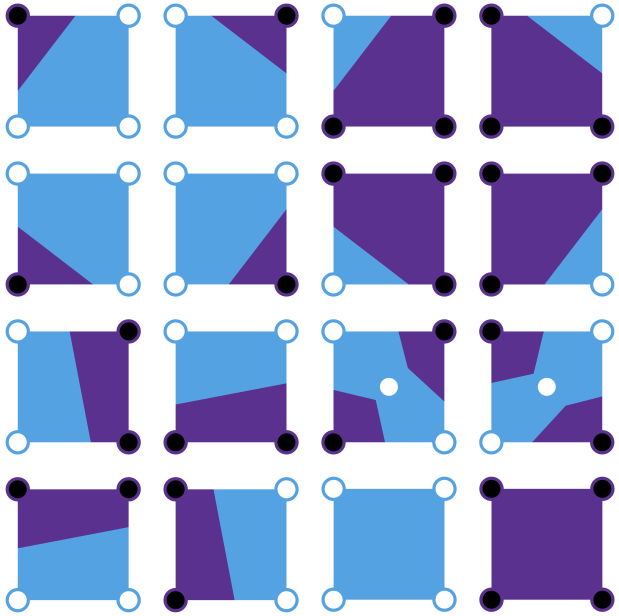
\includegraphics[scale=0.32]{img/Marching_squares_isolines.svg.png}
    \caption{Sedici casi possibili in cui possono ricadere i quadrati composti dai quattro valori.}
\end{figure}
\begin{figure}[H]
    \centering
    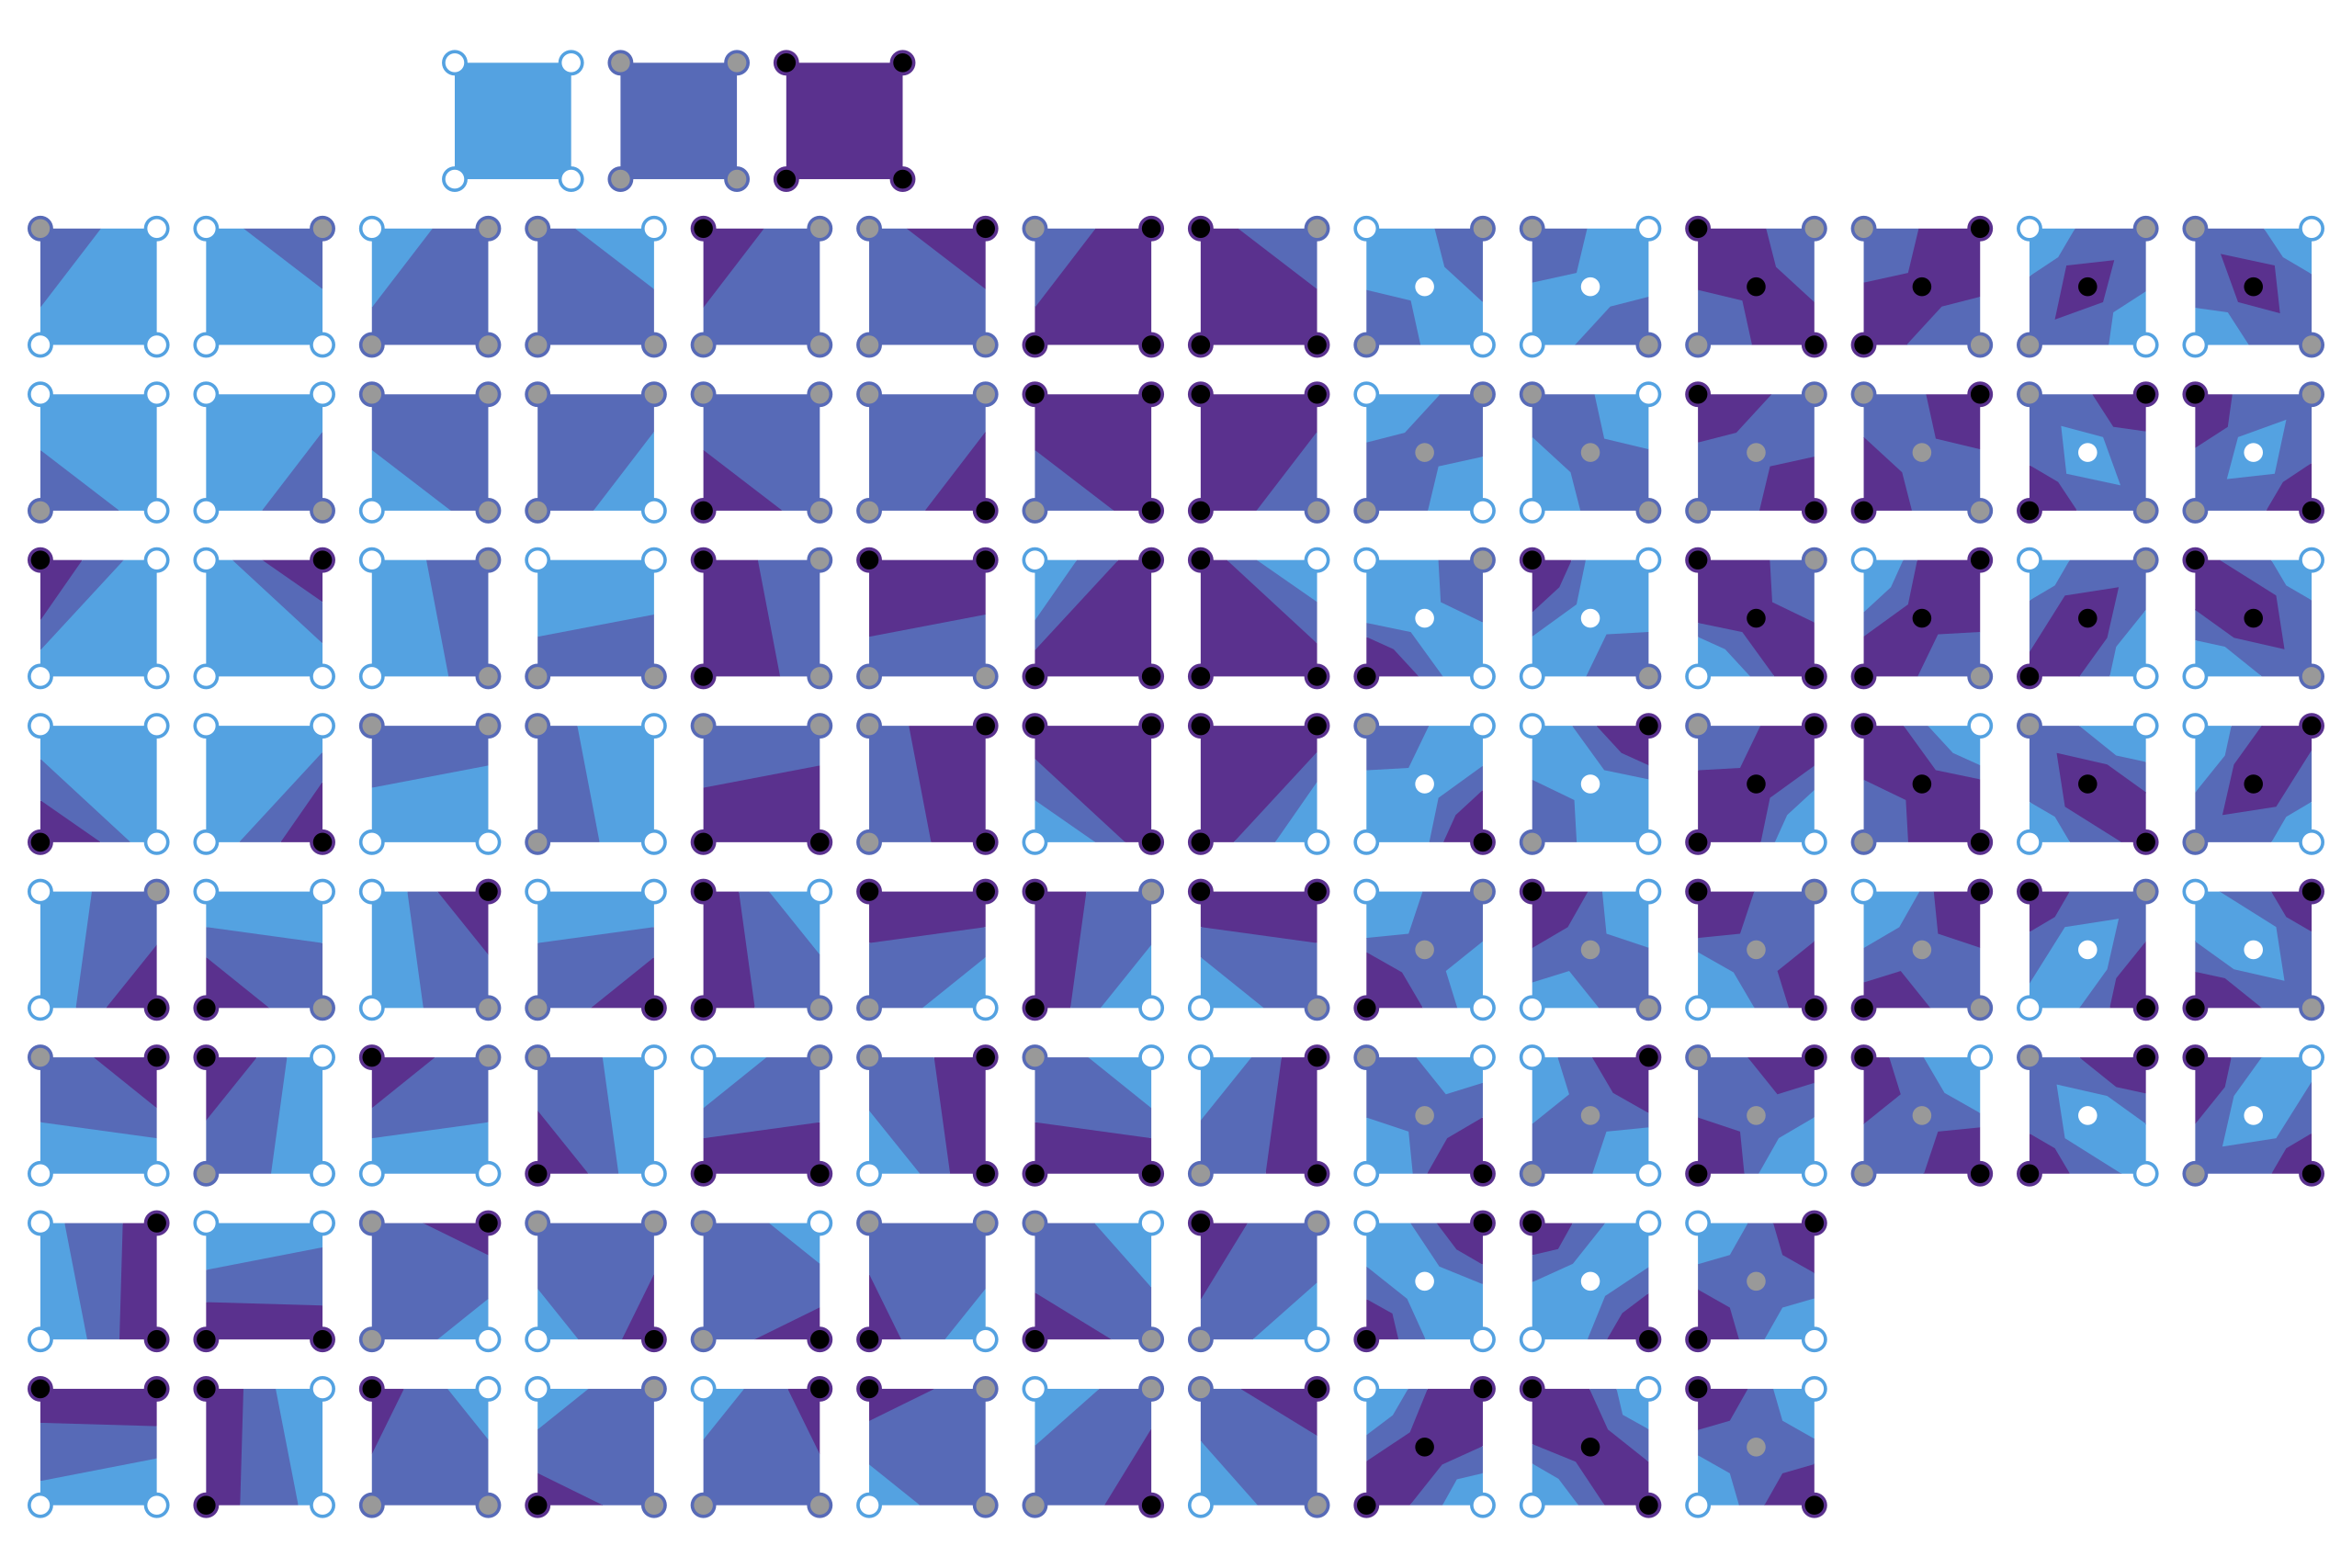
\includegraphics[scale=0.17]{img/Marching_squares_isobands.svg.png}
    \caption{Casi possibili nella versione con isobande in cui possono ricadere i quadrati composti dai quattro valori.}
\end{figure}

%embarrassingly parallel
% problema di classificazione tipo in modo indipendente ma ricostruzione contorno unito in modo seriale/congiunto
L'algoritmo é embarrassingly parallel per quanto riguarda la classificazione per tipo di ogni cella (quadrato con valori negli spigoli) poiché puó essere svolta in modo indipendente tra le celle. \newline
La fase di ricostruzione dei contorni invece può essere svolta sia in parallelo che in seriale utilizzando tecniche e modalità differenti che dipendono dall'utilizzo finale a cui il codice é destinato. \newline
%utilizzi reali, utilitá
MS è utilizzato per molte applicazioni pratiche in settori di particolare interesse come ad esempio:
\begin{itemize}
\item Computer Graphics per generare immagini 3D da dati 2D.
\item Rilevamento remoto in immagini satellitari o radar.
\item Medicina per analizzare scansioni CT o immagini MRI dove possono essere identificare anomalie come tumori.
\item Scienze naturali per l'analisi di dati meteorologici e oceanici nell'identificazione di aree di pioggia o di correnti forti.
\item Cartografia per la generazione di mappe relative a paesi o città da dati 2D.
\end{itemize}

\subsection{Problema Reale}
Bioretics è l'azienda con cui è stara svolta la ricerca, uno dei settori in cui opera è quello della selezione automatica della frutta. La selezione della frutta è un processo svolto in questo caso da macchine dotate di rulli e fotocamere, i frutti entrano nella macchina all'interno di tazze e vengono fatti roteare da dei rulli in modo da poter acquisire con delle camere fissate all'interno della macchina delle immagini di tutta la superficie dei frutti. Le immagini scattate per ogni frutto vengono processate e passate ad una CNN che restituisce delle matrici della stessa dimensioni delle immagini scattate, una per ogni classe di difetto che si vuole valutare, che hanno come valore la probabilità che il rispettivo pixel appartenga a quella classe. \newline

L'azienda offre in sostanza un prodotto software che viene eseguito da macchine per la selezione della frutta e include l’utilizzo dell'algoritmo Marching Squares (MS). La sfida proposta dall'azienda è quella di ridurre i tempi di esecuzione di MS che è utilizzato nella fase di segmentazione dei difetti.
Le macchine per la selezione gestiscono un flusso di circa 10 frutti al secondo, ne consegue che ci sia approssimativamente 0.1s a disposizione per ogni frutto. Quindi un’implementazione parallela dell’algoritmo MS, che riesca a ottenere uno speedup anche solo di 1.1 sarebbe considerato un risultato positivo per l’azienda.
Scendendo più nel merito degli aspetti tecnici, all’interno delle macchine vengono scattate immagini dei frutti da camere fissate e calibrate che sono poi elaborate da una CNN che a sua volta restituisce un tensore WxHxC, dove ogni canale rappresenta una classe (esempio: picciolo, ammaccatura, muffa). I canali vengono poi passati singolarmente al MS che definisce i contorni di ogni classe in base ad un valore di soglia specificato. Il risultato del processo è visibile dall’immagine della figura 3.3 dove si possono notare le varie classi delimitate da colori differenti. \newline

\begin{figure}[H]
    \centering
    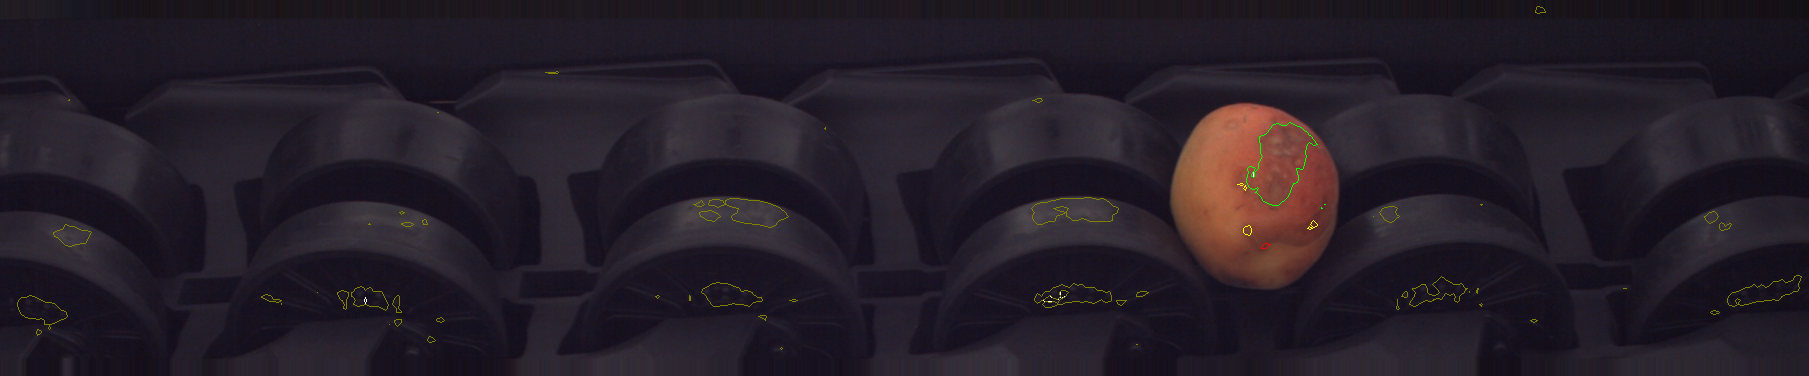
\includegraphics[scale=0.25]{img/marching_squares_00000052_00000001.png}
    \caption{Immagine scattata da macchina per la selezione della frutta senza elaborazioni applicate.}
\end{figure} 

L’implementazione di MS che è attualmente utilizzata dall’azienda deriva dalla libreria scikit-image che offre una versione seriale dell’algoritmo. Il metodo della libreria che viene chiamato è scritto in Python ma la parte principale è stata scritta in Cython.
Il codice in Cython deve essere compilato prima di essere eseguito, nel complesso però riduce i tempi di esecuzione rispetto all’equivalente in Python. Bisogna quindi considerare che il tempo totale di esecuzione di MS è stato già in parte ridotto dagli autori della libreria. \newline
In tutte le macchine sulle quali esegue il codice dell'azienda sono montate schede video di fascia alta per quanto riguarda le prestazioni, l'utilizzo di codice parallelo su GPU può essere quindi ampiamente sfruttato per ridurre i tempi di esecuzione e sollevare del carico la CPU su cui altrimenti ricadrebbe con esecuzioni seriali che in confronto sono estremamente dispendiose in termini di tempo.

\subsection{Obbiettivo}
L'obbiettivo concordato con l'azienda è quello di implementare una versione parallela su GPU (scheda video) dell'algoritmo Marching Squares, l'ottenimento di uno speedup rispetto alla versione utilizzata attualmente ovvero il metodo \verb|findContours| della libreria skimage sarebbe considerata un successo. \newline
Il software dell'azienda che attualmente richiama la funzione \verb|findContours| è scritta in Python, è necessario quindi riuscire trovare un metodo per poter sfruttare l'esecuzione parallela su GPU da Python, operazione non comune dato che solitamente i kernel Cuda sono lanciati da codice C o C++ ovvero a un livello di astrazione molto più basso di Python e con strutture dati come puntatori compatibili con quelli di Cuda. \newline
L'implementazione finale può essere rappresentata dallo schema in figura 3.4 ovvero una componente software che può essere richiamata direttamente da codice Python cioè un altro componente Python e delle parti aggiuntive di codice più a basso livello che siano in grado di lanciare ed eseguire codice sulla GPU in parallelo. L'unica parte della soluzione per cui la scelta del linguaggio da utilizzare risulta automatica è quella con cui si interfaccerà il codice dell'azienda, sarà quindi un modulo Python da cui poi si cercherà una strategia per arrivare all'esecuzione su GPU. \newline


\begin{figure}[H]
    \centering
    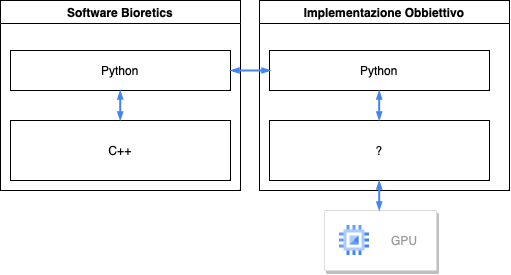
\includegraphics[scale=0.8]{img/Diagram_Python_GPU.drawio.png}
    \caption{Schema linguaggi utilizzati dal software dell'azienda e da utilizzate per la soluzione finale.}
\end{figure}

\section{Analisi implementazione skimage}
% analisi del metodo findContours
Il metodo \verb|findContours| di skimage composto da due fasi principali, nella prima viene richiamato un metodo \verb|_get_contour_segments| che trova le coordinate dei segmenti che costituiscono i contorni e una seconda parte in cui viene richiamato \verb|_assemble_contours| che dall'output di \verb|_get_contour_segments| unisce i segmenti che si intersecano sui bordi delle celle formando linee spezzate. \newline
% analisi parte core in Cython
Il metodo \verb|_get_contour_segments| è contenuto nel file \verb|_find_contours_cy.pyx| che è scritto in codice Cython, questo linguaggio è un superset di Python che permette di scrivere codice Python-like che effettua chiamate a funzioni C e può dichiarare tipi di dato del C, queste caratteristiche permettono al compilatore di generare codice ottimizzato per quanto riguarda i tempi di esecuzione rispetto all'equivalente in Python. \newline
% confronto prestazione Python<-->Cython
Non è semplice stabilire lo speedup del codice Cython rispetto al Python poiché il confronto dipende fortemente dalle strutture dati usate, il numero di funzioni C e python richiamate e altri fattori che influiscono in maniera significativa sulla differenza tra i tempi di esecuzione dei due linguaggi. Indubbiamente le chiamate a funzioni C da codice Cython introducono un overhead rispetto alla stessa chiamata effettuata da C e le funzioni Python impiegano un tempo sicuramente al massimo uguale e sicuramente non minore delle stesse funzioni richiamate da codice Python nativo. \newline
Nel complesso però se il codice Cython viene scritto con particolari accortezze nell'utilizzo di soli tipi di dato C e richiamando funzioni Python solo se indispensabili il codice che ne deriva risulta estremamente più veloce della versione Python, con tempi di esecuzione si avvicinano alla versione C che teoricamente può essere considerata un suo lower bound. Queste osservazioni sono riscontrabili graficamente nei risultati dei test generici riportati nella figura 3.5. 
\begin{figure}[H]
    \centering
    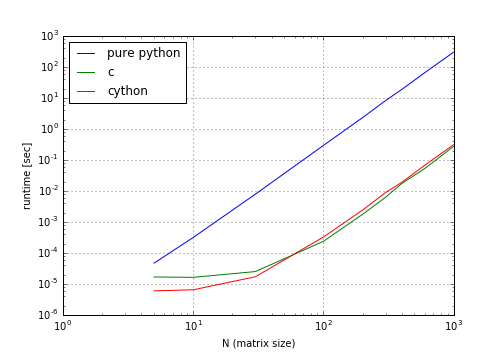
\includegraphics[scale=0.9]{img/cython-vs-c.png}
    % Image Source: http://ibm.co/20XSZ4F
    \caption{Grafico che mette in comparazione i tempi di esecuzione di Pyhon, C e Cython su un task di esempio. 
%TODO valutare di rifarlo manualmente o trovare altra fonte]
}
\end{figure} \newpage
Il codice del metodo Cython \verb|_get_contour_segments| risulta particolarmente ottimizzato in quanto utilizza unicamente variabili di tipo C e richiama una sola funzione di Python ovvero \verb|append| che può essere eseguita solitamente 0,1 o al massimo 2 volte per ogni quadrato considerato. 
% osservazine --> tempi libreria già stretti
Il codice del metodo findContours può essere considerato quindi già particolarmente ottimizzato per essere un metodo Python, in quanto il suo tempo di esecuzione si può avvicinare molto ad una versione scritta in C. \newline
Con una immagine 511x95 il metodo findContours impiega in media circa \verb|0.0024s|**[NOTA: sulla mia macchina,  attendo test su server azienda per aggiornare valore e inserire specifiche macchina] %TODO specifiche macchina
ovvero neanche tre millesimi di secondo.

\section{Limiti della programmazione parallela}
% intro generale ai problemi della prog parallela
% spiegare che parte più dispendiosa in questo caso sarebbe caricamnto e scrittura dati visto che l'esecuzione di immagini di queste dimensioni è esigua
% osservazione --> dimensioni immagini
Nelle architettura Von Neumann la latenza introdotta dagli accessi alla memoria sono ordini di grandezza maggiori rispetto a un ciclo di clock e creano bottleneck che influiscono molto sui tempi di esecuzione di una versione di codice parallela.
Nell'applicazione pratica proposta dall'azienda le immagini da elaborare sono di dimensioni 511x95, con una versione parallela del Marching Squares idealmente ogni Cuda Core si occuperebbe di un singolo quadrato, con immagini di queste dimensioni servirebbero 47940 esecuzioni (ovvero il numero di quadrati) che una GPU di fascia alta riesce a coprire utilizzando tutti i suoi Cuda Core in parallelo reiterando il procedimento qualche volta. \newline
Indipendentemente da come può essere gestito il lancio e l'esecuzione del MS su GPU è indispensabile che l'immagine sia letta dalla memoria principale della macchina, caricata sulla memoria della GPU e in seguito il processo opposto sul risultato ottenuto sulla GPU.
Queste operazioni di trasferimento dati tra memorie sono estremamente dispendiose paragonate ai tempi di esecuzione delle istruzioni che un kernel Cuda può impiegare, questo rischia di essere uno dei maggiori problemi e limiti da affrontare per raggiungere uno speedup in quanto sicuramente una versione di codice parallelo ha il potenziale di essere più veloce del rispettivo seriale, ma al tempo del codice parallelo va sommato il tempo per caricare e scaricare i dati dalla GPU che influiranno in gran parte sul tempo di esecuzione finale. \newline
Se l'immagine fosse di dimensioni maggiori il tempo dovuto al bottleneck potrebbe essere ammortizzato maggiormente e la versione parallela avrebbe più margine su quella seriale, nel nostro caso invece la grandezza dell'immagine non richiede un tempo di esecuzione sufficientemente grande da far passare in secondo piano quello dei trasferimenti tra memorie. \newline
Il caso peggiore che si può presentare è che il rapporto dati da trasportare e le operazioni da effettuarci sia così sbilanciato che solamente il tempo di upload e download dei dati dalla GPU senza neanche contare il tempo di esecuzione del codice parallelo sia maggiore del tempo di esecuzione della versione seriale.


\section{Analisi versione seriale di MS}
La libreria \verb|scikit-image| (skimage) è un pilastro per quanto riguarda l'elaborazione di immagini in ambito Open-Source, è largamente utilizzata sia in piccoli progetti che in contesti industriali.  Il codice delle funzioni più utilizzate è particolarmente solido e ottimizzato pur mantenendo un'ampia compatibilità con una vasta lista di ambienti, tra queste funzioni ricade anche findContours che infatti presenta ottime prestazioni per essere una funzione seriale lanciata da Python.\newline
Dal codice di findContours che è riportato nella sezione di codice 1, proveniente dal file \verb|scikit-image/skimage/measure/_find_contours.py|, si può notare facilmente che vengono richiamati due metodi \verb|_get_contour_segments| e \verb|_assemble_contours| che costituiscono le due fasi di costruzione del risultato, la prima di pura ricerca algoritmica dei segmenti che costituiscono i contorni e la successiva di congiunzione dei contorni confinanti in linee spezzate. \\[10pt]
\noindent\rule[0.5ex]{\linewidth}{2pt}
\small{\textbf{Codice 1: Metodo find\_contours di scikit-image}} \\
\noindent\rule[0.5ex]{\linewidth}{1pt}

\lstset
{ %Formatting for code in appendix
    language=Python,
    basicstyle=\footnotesize,
    numbers=left,
    stepnumber=1,
    showstringspaces=false,
    tabsize=1,
    breaklines=true,
    breakatwhitespace=false,
}
\begin{lstlisting}
def find_contours(image,  level=None,  fully_connected='low', 
																		positive_orientation='low', *,  mask=None):

					...
					# parameters configuration
					...	

					segments = _get_contour_segments(
					 			image.astype(np.float64), 
					 			float(level),
								 fully_connected == 'high', 
					 			mask=mask)
    	contours = _assemble_contours(segments)
    	if positive_orientation == 'high':
        		contours = [c[::-1] for c in contours]
    	return contours
\end{lstlisting}
\noindent\rule[0.5ex]{\linewidth}{1pt} \\[10pt]
Il metodo \verb|_get_contour_segments| non è compreso nello stesso modulo di  \verb|find_contours| ma nel file \verb|scikit-image/skimage/measure/_find_contours_cy.pyx| che come si può notare termina con \verb|.pyx|, estensione che contraddistingue file contenenti codice Cython.  Come già accennato infatti \verb|_get_contour_segments| è stato scritto in Cython poiché è la parte computazionalmente più impegnativa dell'intero metodo \verb|find_contours|.  \newline
La maggior parte dei tipi di dati sono derivati dal C++ e altri dal Python come riportato nel seguente estratto di codice 2 del metodo Cython.  \newpage
\noindent\rule[0.5ex]{\linewidth}{2pt}
\small{\textbf{Codice 2: Estratto dal Metodo \_get\_contour\_segments di scikit-image}} \\
\noindent\rule[0.5ex]{\linewidth}{1pt}
\begin{lstlisting}
cimport numpy as cnp
cnp.import_array()
cdef extern from "numpy/npy_math.h":
    bint npy_isnan(cnp.float64_t x)
cdef list segments = []
cdef bint use_mask = mask is not None
cdef unsigned char square_case = 0
cdef tuple top, bottom, left, right
cdef cnp.float64_t ul, ur, ll, lr
cdef Py_ssize_t r0, r1, c0, c1
\end{lstlisting}
\noindent\rule[0.5ex]{\linewidth}{1pt} \\[10pt]
L'utilizzo dei questi tipi di dato C++ rispetto ai tipi Python permette di ottenere una compilazione più aderente alle necessità e volontà del programmatore che può specificare in modo preciso i tipi di dato di cui necessita. \newline
La porzione di codice più importante del metodo \verb|_get_contour_segments| è costituita da due cicli for annidati che scorrono tutta la matrice in input e considerano un quadrato di 4 celle ad ogni iterazione,  calcolano a quale dei sedici diversi tipi appartiene e aggiornano una struttura dati contenente tutti segmenti dei contorni trovati. \newline
Nell'aggiornamento dei segmenti trovati possono presentarsi tre diversi casi per quanto riguarda il numero di segmenti trovati:
\begin{itemize}
\item 0 segmenti da aggiungere: per i tipi 0 e 15 che sono quadrati con i 4 spigoli rispettivamente sotto e sopra la soglia di threshold non è necessario aggiungere alcun segmento poiché la relativa sezione dell'immagine in questione è completamente esclusa o inclusa in una certa classe,  non è attraversata quindi da segmenti del contorno come si può vedere dalla figura 3.6.
\begin{figure}[H]
\centering
\begin{floatrow}[1]
    \ffigbox[\FBwidth]{\caption{\small{Caso 0 e 15 dell'algoritmo Marching Squares.}}}{
\includegraphics[scale=0.27]{img/Case_0_15.svg.png}}
\end{floatrow}
\end{figure}
\item 2 segmenti da aggiungere: per i tipi 6 e 9 che sono quadrati con le due coppie di spigoli opposti in cui una è maggiore e una minore della soglia.  In questi due casi i segmenti da disegnare sono due,  ci sono due aree appartenenti ad una certa classe che hanno contorni vicini ma separati come osservabile nella figura 3.7.
\begin{figure}[H]
\centering
\begin{floatrow}[1]
    \ffigbox[\FBwidth]{\caption{\small{Caso 6 e 9 dell'algoritmo Marching Squares.}}}{
\includegraphics[scale=0.27]{img/Case_6_9.svg.png}}
\end{floatrow}
\end{figure}

\item 1 segmento da aggiungere: tutti gli altri tipi esclusi 0, 15, 6 e 9 hanno solamente un segmento che li attraversa in diverse modalità con diverse configurazioni di valori per i quattro spigoli del quadrato.  Rappresentano i casi più comuni di aree di contorno e   solitamente compongono la porzione maggiore di segmenti di cui sono costituite le linee spezzate con cui viene disegnato il contorno. Le 12 configurazioni sono rappresentate nella figura 3.8.
\begin{figure}[H]
\centering
\begin{floatrow}[1]
    \ffigbox[\FBwidth]{\caption{\small{Casi 1-5,7,8,10-14 dell'algoritmo Marching Squares.}}}{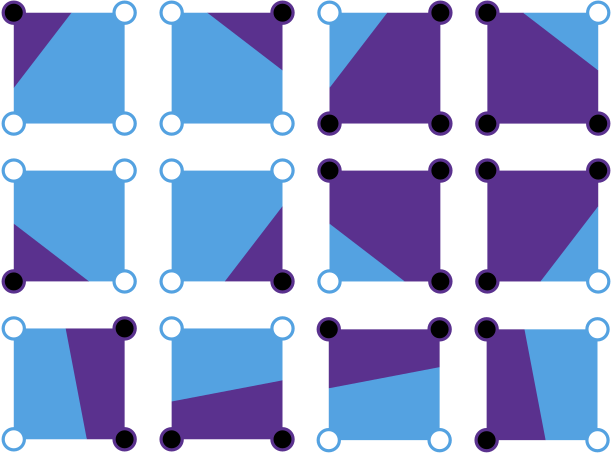
\includegraphics[scale=0.27]{img/Case_1seg.svg.png}}
\end{floatrow}
\end{figure}

\end{itemize}
% spiegare codice Cython per algoritmo MS
Ad ogni iterazione una volta definito a quale tipo appartiene un quadrato vengono aggiunti alla lista \verb|segments| i relativi segmenti trovati che possono essere 0, 1 o 2 come appena specificato.  Per ogni segmento trovato viene aggiunta a  \verb|segments| una tupla contenente altre due tuple in cui sono memorizzate le coordinate x e y del punto di inizio e fine del segmento, nel seguente estratto del metodo  \verb|_get_contour_segments| (Codice 3) viene riportata l'assegnazione delle coordinate per i punti che potranno essere aggiunti alla lista come estremi dei segmenti individuati.\newpage
\noindent\rule[0.5ex]{\linewidth}{2pt}
\small{\textbf{Codice 3: Estratto dal Metodo \_get\_contour\_segments di scikit-image}} \\
\noindent\rule[0.5ex]{\linewidth}{1pt}
\begin{lstlisting}
cdef inline cnp.float64_t _get_fraction(cnp.float64_t from_value,
                                        cnp.float64_t to_value,
                                        cnp.float64_t level):
    if (to_value == from_value):
        return 0
    return ((level - from_value) / (to_value - from_value))

top = r0, c0 + _get_fraction(ul, ur, level)
bottom = r1, c0 + _get_fraction(ll, lr, level)
left = r0 + _get_fraction(ul, ll, level), c0
right = r0 + _get_fraction(ur, lr, level), c1
\end{lstlisting}
\noindent\rule[0.5ex]{\linewidth}{1pt} \\[10pt]
Ognuno dei 16 casi deve essere gestito separatamente poiché le loro composizioni sono eterogenee per quanto riguarda i valori sugli spigoli e le coordinate da salvare.  
I segmenti vengono aggiunti alla lista  \verb|segments| tramite la funzione  \verb|append| che permette di costruire la lista di segmenti finale in modo incrementale senza dover conoscere a priori quale sarà la lunghezza finale della lista o quanti segmenti sarà necessario scrivere per ogni quadrato.  Per i casi 0 e 15 non è necessario aggiungere nessun segmento a segments quindi si passa direttamente all'iterazione successiva, per gli altri casi invece si aggiungono 1 o 2 segmenti in base al caso in cui si ricade.\\[10pt]
\noindent\rule[0.5ex]{\linewidth}{2pt}
\small{\textbf{Estratto dal Metodo \_get\_contour\_segments di scikit-image}} \\
\noindent\rule[0.5ex]{\linewidth}{1pt}
\begin{lstlisting}
# Manage case 0 and 15
if square_case in [0, 15]:
                continue

# Example for case 1-5, 7, 8, 10-14
if (square_case == 1): 
                # top to left
                segments.append((top, left))
# Example for case 6 and 9
elif (square_case == 6):
                 segments.append((left, top))
                 segments.append((right, bottom))
\end{lstlisting}
\noindent\rule[0.5ex]{\linewidth}{1pt} \newpage

% spiegare problema append per la parallelizzazione su GPU e le strutture dati
\subsection{Predisposizione alla parallelizzazione}
L'algoritmo Marching Squares essendo embarassingly parallel è teoricamente predisposto ad una parallelizzazione, le soluzioni parallele però hanno necessità specifiche che il codice seriale non ha bisogno di rispettare,  per riuscire a raggiungere questi requisiti partendo dal codice di  \verb|_get_contour_segments| è necessario effettuare radicali modifiche alle strutture dati utilizzate e al loro utilizzo. \newline
La principale criticità riscontrabile nel metodo è l'utilizzo di una lista e del metodo \verb|append| che non è possibile trasformare direttamente in ad esempio codice di un kernel Cuda poichè la dimensione finale della lista non è nota a priori e il metodo  \verb|append| non è disponibile in Cuda.  La funzione \verb|append| non potrebbe neanche essere utilizzata in una versione parallela ottimizzata poiché implica un accesso serializzato alla struttura dati lista per aggiungere il nuovo elemento in una nuova e ultima posizione della lista, questa operazione non può quindi essere effettuata contemporaneamente da più Cuda Core.  Per una versione parallela su GPU dato che il tipo dei quadrati e l'aggiunta dei segmenti verrebbe eseguita contemporaneamente sarebbe necessario avere un accesso indipendente e non vincolato alla risorsa di output su cui scrivere,  questo comporta la necessità di una struttura dati con un numero di posizioni già definito ma anche il numero di segmenti che ogni Cuda Core (ovvero per ogni quadrato valutato) necessita di scrivere.

% \chapter{Tentativi Svolti}
% valutare cambio nome
% spiegare tutti i tentativi svolti, 1 o più capitoli per ogni veersione o test
\chapter{Versione parallela con nvc++} 
La prima strategia esplorata consiste nel compilare il codice Cython con le ultime versioni del compilatore nvc++ che supportano dei flag per la parallelizzazione automatica su GPU.  Nvidia ha recentemente aggiornato \verb|stdpar,|  un flag che promette di riuscir a parallelizzare automaticamente codice C++ su GPU utilizzando il compilatore nvc++. \newline
Il processo parte da del codice Cython che tramite il proprio compilatore viene trasformato in codice C++,  a questo punto si compila il codice C++ utilizzando nvc++ e una serie di flag per la parallelizzazione parallela compreso \verb|stdpar|. \newline
Il processo completo documentato da Nvidia è descritto nella figura 4.1.
\begin{figure}[H]
\centering
\begin{floatrow}[1]
    \ffigbox[\FBwidth]{\caption{\small{Schema di descrizione processo per utilizzo nvc++ in parallelizzazione codice Cython prodotto a Nvidia.}}}{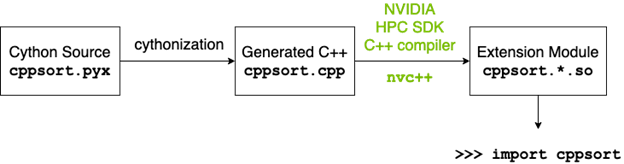
\includegraphics[scale=0.9]{img/extension-module.png}}
\end{floatrow}
\end{figure}

\section{Risultati ottenuti}
 

\chapter{Versione parallela con API Cuda-Python} 
% problema dell'append in Cython non convertibile direttamente in Cuda ==> utilizzo array
% tecnica innovativa exclusive scan
\section{Risultati ottenuti}


\chapter{Risultati a Confronto}
% speedup, ecc.. In sostanza si descrivono e commentano i grafici ottenuti
% se si vuole misurare tempo di 2° paarte di find_contours() poi meglio lasciare distinte le due misurazioni (lib completa e assemble contours) in modo di dare a chi legge la possibilità di valutare la precisione non perfetta della misura

\chapter{Conclusioni}
% speculare all'abstract, si dicono le stesse cose ma invece che "andremo a fare"  si dirà "abbiamo fatto"
% keyword: ABBIAMO fatto

\end{document}
